\documentclass[12pt]{article}
\usepackage{fontspec}
\usepackage{polyglossia}
\usepackage{geometry}
\usepackage{xcolor}
\usepackage{titlesec}
\usepackage{fancyhdr}
\usepackage{graphicx}
\usepackage{mathtools}
\graphicspath{{../matlab/figures/}}
\usepackage{hyperref} % Add hyperref package for clickable links
\usepackage{amsmath}
\usepackage{tabularx}

\usepackage{float}
\usepackage{caption}
\usepackage{subcaption}



% Set the page margins
\geometry{margin=2.54cm}

%\usepackage{kmath,kerkis} % The order of the packages matters; kmath changes the default text font
%\usepackage[T1]{fontenc}

% Set the font to Kerkis
\setmainfont{Calibri}


\usepackage{matlab-prettifier}
\newfontfamily\greekfonttt[Script=Greek]{Calibri}

% Define colors
\definecolor{myblue}{RGB}{0, 51, 102}
\definecolor{mygray}{RGB}{150,150,150}
\definecolor{mybg}{RGB}{230,230,230}

% Set section title formatting
\titleformat{\section}
  {\normalfont\Large\bfseries\color{myblue}}
  {\thesection}{1em}{}
%\titleformat{\subsection}
%  {\normalfont\Large\bfseries\color{myblue}}
%  {\thesubsection}{1em}{}

\setmainlanguage{greek}
\setotherlanguage{english}

% Define header and footer
\pagestyle{fancy}
\fancyhf{}
\lhead{Ομάδα 2}
\rhead{Υλοποίηση εξελικτικού πρωταθλήματος Axelrod}
\rfoot{\thepage}

%\title{Αναφορά εργαστηρίου}
%\author{Όνομα Φοιτητή}
%\date{\today}

\begin{document}
\begin{titlepage}
\newgeometry{margin=2cm, tmargin=3cm, bmargin=3cm}
\centering
\begin{figure}[H]
\centering

\includegraphics[width=0.8\textwidth]{banner-horizontal-black300ppi.png}\par % Image on top of title
\end{figure}
%\textcolor{black}{\large \bfseries Αριστοτέλειο Πανεπιστήμιο Θεσσαλονίκης\\}\par
\vspace{18pt}
\textcolor{black}{\Large \bfseries Τμήμα Ηλεκτρολόγων Μηχανικών\\και Μηχανικών Υπολογιστών\\}\par
\vspace{1cm}
\vfill
\textcolor{black}{\Large \bfseries Θεωρία Παιγνίων}\par
\vspace{12pt}
\textcolor{black}{\large \bfseries Υλοποίηση εξελικτικού πρωταθλήματος Axelrod}\par

\vspace{0.5cm} % Adjust vertical spacing here
\vfill
\newcolumntype{L}{>{\raggedright\arraybackslash}X}%
\newcolumntype{R}{>{\raggedleft\arraybackslash}X}%
{\large
\def\arraystretch{1.3}
\begin{tabularx}{\textwidth}{ R|L }
\textbf{Ομάδα}                			 & 2           \\
\textbf{Βαπόρης Δημήτριος}      & ΑΕΜ 10625 \\
\textbf{Βουλκίδης Βλάσιος}        & ΑΕΜ 10627 \\
\textbf{Ντελόπουλος Εμμανουήλ}      & ΑΕΜ 10693 \\
\textbf{Υπεύθυνος Καθηγητής}           & Κεχαγιάς Αθανάσιος\\
\end{tabularx}
}
\vspace{0.5cm}
\vfill
\textcolor{black}{\large \bfseries Εαρινό Εξάμηνο 2025}\par
\end{titlepage}
\restoregeometry

\tableofcontents % Table of Contents

\newpage
\section{Εισαγωγή}
Το συγκεκριμένο αρχείο είναι η αναφορά της εργασίας για το μάθημα Θεωρία Παιγνίων. Αντικείμενο της εργασίας αυτής είναι η υλοποίηση και η μελέτη του εξελικτικού πρωταθλήματος Axelrod στο παίγνιο "Δίλημμα του Φυλακισμένου". Με την ονομασία αυτή χαρακτηρίζεται το κοινωνικό δίλημμα, δηλαδή οποιοδήποτε παίγνιο της μορφής $\begin{bmatrix} A_{1,1} & A_{1,2} \\ A_{2,1} & A_{2,2} \end{bmatrix}$, τιμές για τις οποίες ισχύει $ A_{1,2} < A_{2,2} < A_{1,1} < A_{2,1}$. Η επανάληψη του παιγνίου αυτού δημιουργεί ένα match μεταξύ στρατηγικών, matches μεταξύ στρατηγικών δημιουργούν τουρνουά μεταξύ στρατηγικών και ο υπολογισμός νέου πληθυσμού με βάση την επίδοση κάθε στρατηγικής στο τουρνουά αποτελεί το αντικείμενο μελέτης της εργασίας. 

Η εργασία αποτελείται από 4 βασικές συναρτήσεις, κάθε μία από τις οποίες επιτελεί μία συγκεκριμένη λειτουργία που μπορεί να χαρακτηριστεί από δύο χαρακτηριστικά της εκάστοτε παραδοχής: η φύση της προσομοίωσης (θεωρητική ή πραγματική) και η εξελικτική δυναμική (fitness ή imitation). Συγκεκριμένη εισαγωγή γίνεται και κατά την παρουσίαση της κάθε συνάρτησης, στην οποία εξηγείται ο τρόπος λειτουργίας και τυχούσες παραδοχές που συνέβησαν σε κάθε περίπτωση. Το πρώτο μέρος της εργασίας βασίζεται σε σημαντικό ποσοστό στη μελέτη των Mathieu et al. Μάλιστα, καταβλήθηκε προσπάθεια τα αποτελέσματα να είναι κατά το δυνατόν όμοια με αυτά που παρουσιάζει το paper του 1999.

\section{Fitness Dynamics}

Πρώτη εξελικτική δυναμική που θα αναλυθεί (και αυτή που αναλύεται από τους Mathieu et al.) είναι η δυναμική του fitness, σύμφωνα με την οποία ανατίθεται σε κάθε στρατηγική της προσομοίωσης ένα score, το οποίο χρησιμοποιείται ώστε να υπολογστεί η κατανομή του πληθυσμού της επόμενης γενιάς. Ακολουθείται και για τις δύο παρακάτω συναρτήσεις που αξιοποιούν το fitness η θεώρηση των Mathieu et al, σύμφωνα με την οποία το fitness κάθε στρατηγικής υπολογίζεται ως εξής: 

Έστω ότι ο πληθυσμός απαρτίζεται από 3 στρατηγικές, την A, την B και την C. Υπολογίζονται με βάση τον πίνακα του παιγνίου B, τον αριθμό των γύρων κάθε αγώνα T και, προφανώς, των στρατηγικών που βρίσκονται "αντιμέτωπες" σε κάθε περίπτωση, οι απολαβές κάθε μίας από τις 2 στρατηγικές και αποθηκεύονται ως π.χ. V(A|B), η απολαβή της στρατηγικής A όταν συναντά την B. Έπειτα, το score κάθε παίκτη που χρησιμοποιεί την εκάστοτε στρατηγική (και άρα, ουσιαστικά, της στρατηγικής) υπολογίζεται ως, π.χ. για τη στρατηγική A, $g_n(A) = W_n(A)V(A|A) + W_n(B)V(A|B) + W_n(C)V(A|C) − V(A|A)$ , όπου $W_n(A), W_n(B), W_n(C)$ οι πληθυσμοί της εκάστοτε στρατηγικής στη γενιά $n$ (παρατηρήστε ότι αφαιρείται μία φορά η απολαβή για παιχνίδι με την ίδια στρατηγική του κάθε παίκτη, διότι θεωρείται ότι παραλείπεται το παιχνίδι με τον εαυτό του κάθε μέλους του πληθυσμού). Τέλος, το συνολικό score του τουρνουά υπολογίζεται ως $t(n) = W_n(A)g_n(A) + W_n(B)g_n(B) + W_n(C)g_n(C)$ και ο πληθυσμός της γενιάς $n+1$ για π.χ. τη στρατηγική A γίνεται $W_{n+1}(A) = \frac{\Pi W_n(A)g_n(A)}{t(n)}$. 

Να επισημανθεί εδώ ότι η λογική αυτή εφαρμόζεται λόγω της πλήρους ντετερμινιστικής φύσης των στρατηγικών που έχουν υλοποιηθεί: εάν υπήρχαν στρατηγικές με τυχαίο στοιχείο, ο θεωρητικός υπολογισμός των αποτελεσμάτων κάθε αγώνα θα ήταν αδύνατος και θα έπρεπε να υπολογιστεί κάποια αναμενόμενη τιμή, αντικείμενο που ξεφεύγει από το αντικείμενο μελέτης της εργασίας.
\subsection{Η συνάρτηση TourSimFit}
Πρώτη συνάρτηση που υλοποιείται είναι η [POP,BST,FIT]=TourSimFit(B,Strategies,POP0,T,J), όπου B ο πίνακας απολαβών του παιγνίου, Strategies ένα array από Strings με τα ονόματα των στρατηγικών που συμμετέχουν στην προσομοίωση, POP0 ο αρχικός πληθυσμός, T ο αριθμός γύρων σε κάθε αγώνα και J ο αριθμός γενεών του εξελικτικού πρωταθλήματος. Επιστρέφονται τα εξής: POP ένας πίνακας με τους πληθυσμούς κάθε στρατηγικής ανά γενεά, BST πίνακας που περιλαμβάνει τις καλύτερες στρατηγικές κάθε γύρου (0 αν δεν ανήκει στις καλύτερες, 1 αν ανήκει στις καλύτερες, οι ισοπαλίες μετράνε) και FIT ένας πίνακας με τα fitness scores κάθε στρατηγικής για κάθε γενεά. Η λογική της συνάρτησης ακολουθεί όσα παρουσιάστηκαν παραπάνω, όμως προστίθεται κατά τον υπολογισμό των πληθυσμών της επόμενης γενιάς λογική ώστε να αποφεύγεται η ύπαρξη δεκαδικών και ο πληθυσμός κάθε στρατηγικής σε κάθε γενιά να παραμένει ακέραιος. Η λογική λειτουργεί ως εξής:

Λαμβάνεται ως αρχικό αποτέλεσμα των παραπάνω πράξεων για τον πληθυσμό το floor των δεκαδικών αποτελεσμάτων. Έπειτα, υπολογίζεται τυχόν έλλειμμα που προκύπτει από την εφαρμογή της συνάρτησης floor και ανατίθεται ένας ανά φορά νέος παίκτης σε κάποια στρατηγική τυχαία, μέχρις ότου να μηδενιστεί το έλλειμμα. Γίνεται και έλεγχος για το αν η στρατηγική βρίσκεται ήδη σε μηδενικό πληθυσμό, ώστε να αποφευχθεί η "αναγέννησή" της. Έτσι, ο συνολικός πληθυσμός των παικτών παραμένει σταθερός καθ' όλη τη διάρκεια της προσομοίωσης, όπως θεωρούν και οι Mathieu et al.

Η επιλογή αυτή γίνεται συνειδητά. Δοκιμάστηκαν οι περιπτώσεις κατά τις οποίες ανατίθεται κάθε παίκτης στη στρατηγική η οποία έχει πληθυσμό πιο κοντά στον επόμενο ακέραιο (π.χ. αν κάποια στρατηγική είχε αρχικά υπολογσιμένο πληθυσμό 199.8, αυτό να μετατραπεί σε 200), όπως και η ακριβώς αντίθετη περίπτωση, όπου δηλαδή ανατίθεται στη στρατηγική πιο μακριά από τον επόμενο ακέραιο. Οι αλγόριθμοι αυτοί παρουσίασαν μερικές ανεπιθύμητες συμπεριφορές διατήρησης ενός πολύ χαμηλού αριθμού παικτών συγκεκριμένων στρατηγικών (π.χ. κάποια στρατηγική να κολλάει σε πληθυσμό 2 επειδή ο αρχικά υπολογισμένος πληθυσμός επόμενης γενεάς είναι 1.8, ή αντίστοιχα π.χ. 1.1). Διατηρώντας αυτό το τυχαίο στοιχείο, τα αποτελέσματα των προσομοιώσεων δεν παρουσιάζουν σημαντική διαφορά με αυτά δίχως τυχαιότητα, ενώ παράλληλα η μέθοδος εγγυάται ότι σε βάθος χρόνου οι "αδύναμες" στρατηγικές εξαφανίζονται πλήρως.

\subsection{Η συνάρτηση TourTheFit}
Η δεύτερη συνάρτηση που υλοποιήθηκε είναι η [POP,BST,FIT]=TourTheFit(B,Strategies,POP0,T,J), με ορίσματα και εξόδους παντελώς πανομοιότυπα με αυτά της προηγούμενης. Η μόνη ουσιαστική διαφορά κείτεται στο ότι πλέον, λόγω της θεωρητικής φύσης της προσομοίωσης, παραλείπεται το τμήμα του κώδικα που ήταν υπεύθυνο για τη διατήρηση ακεραίων στον πληθυσμό, καθώς επιτρέπονται και οι δεκαδικοί αριθμοί, αφού ο πληθυσμός δεν αποτελείται πραγματικά από παίκτες.

\subsection{Προσομοίωσεις}
\subsubsection{1η Προσομοίωση - Defectors may be strong}
	\begin{figure}[H]
	      \centering
	      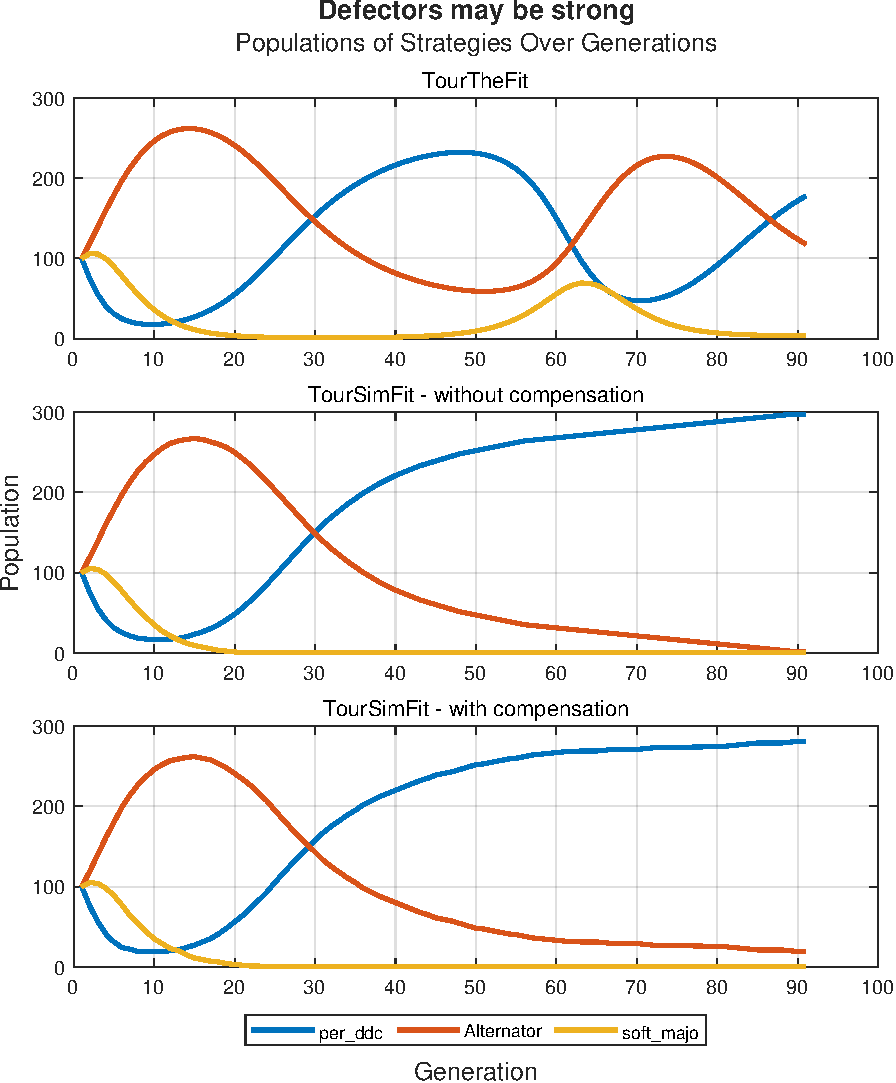
\includegraphics{Defectors may be strong.pdf}
	      \caption{Defectors may be strong}
	      \label{fig:2dmesh}
	\end{figure}
\subsubsection{2η Προσομοίωση - Μονότονη Σύγκλιση}
	\begin{figure}[H]
	      \centering
	      \includegraphics{Monotonous Convergence.pdf}
	      \caption{Monotonous Convergence}
	      \label{fig:2dmesh}
	\end{figure}
\subsubsection{3η Προσομοίωση - Φθίνουσες Ταλαντώσεις}
	\begin{figure}[H]
	      \centering
	      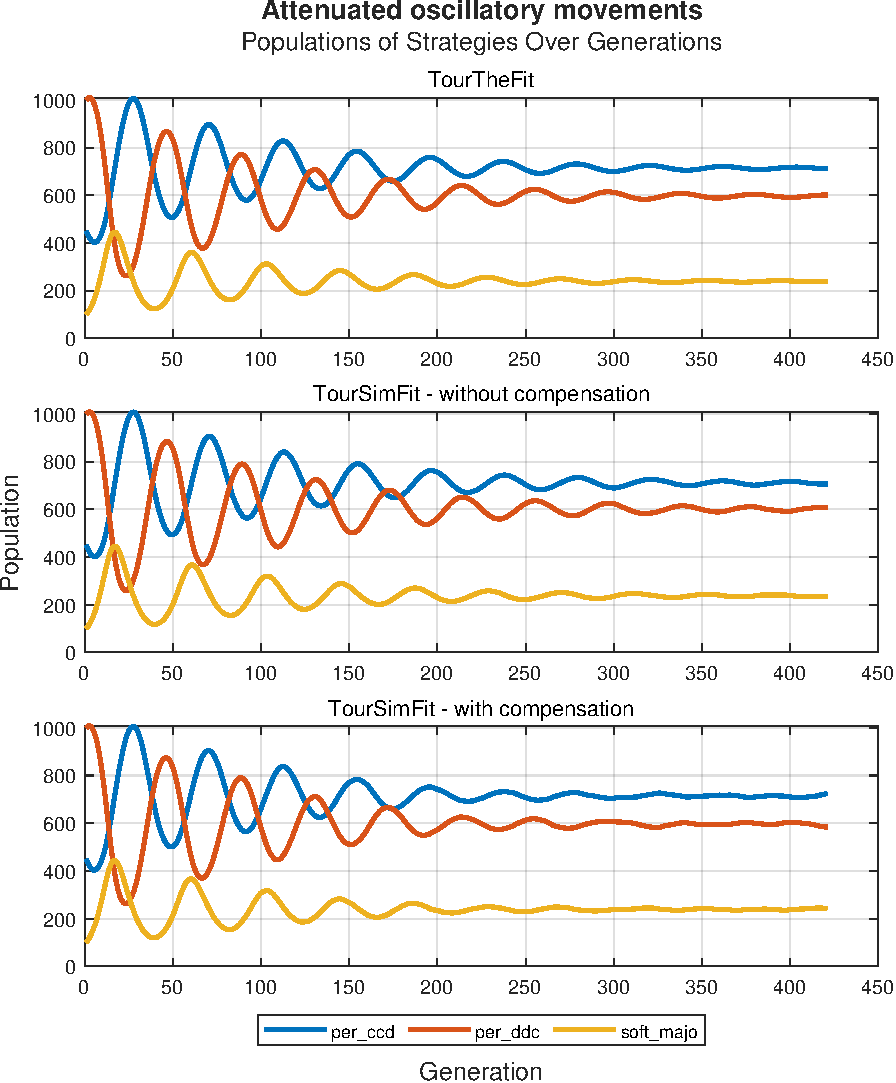
\includegraphics{Attenuated oscillatory movements.pdf}
	      \caption{Attenuated oscillatory movements}
	      \label{fig:2dmesh}
	\end{figure}
\subsubsection{4η Προσομοίωση - Περιοδικές Κινήσεις}
	\begin{figure}[H]
	      \centering
	      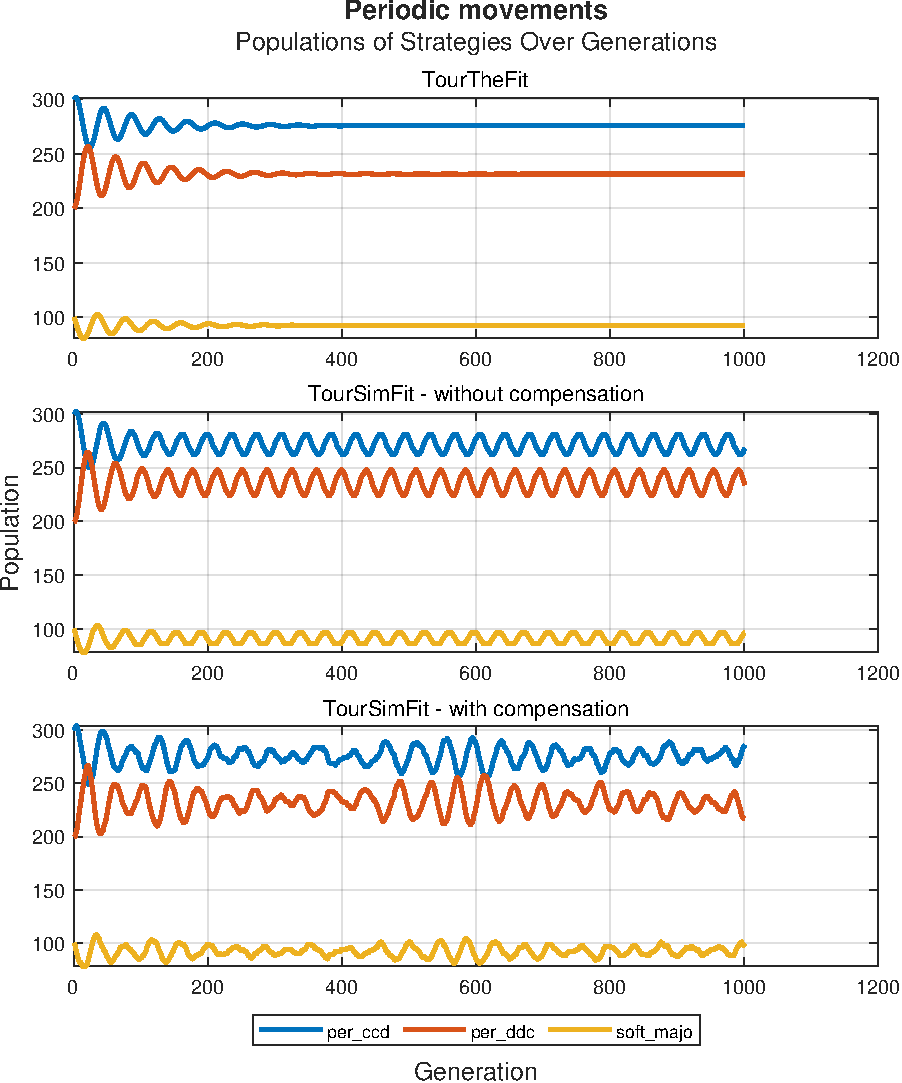
\includegraphics{Periodic movements.pdf}
	      \caption{Periodic movements}
	      \label{fig:2dmesh}
	\end{figure}
\subsubsection{5η Προσομοίωση - Αύξουσες Ταλαντώσεις}
	\begin{figure}[H]
	      \centering
	      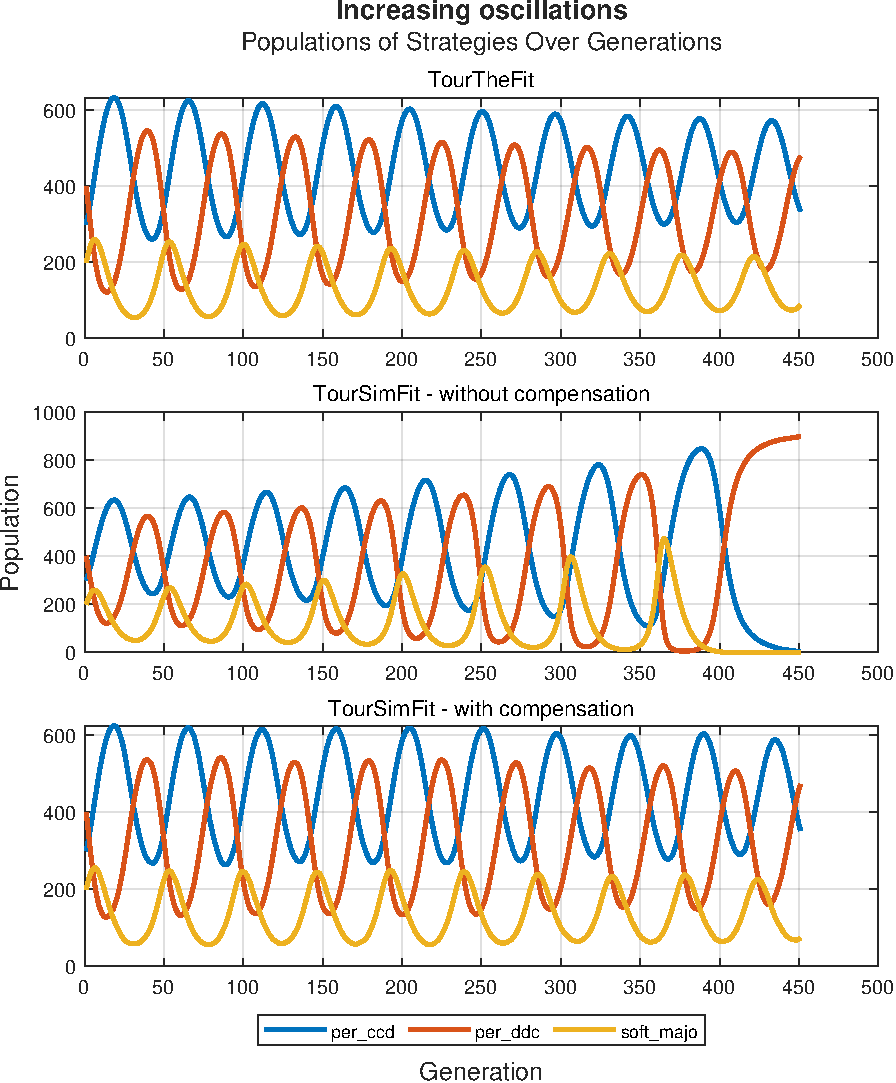
\includegraphics{Increasing oscillations.pdf}
	      \caption{Increasing oscillations}
	      \label{fig:2dmesh}
	\end{figure}
\subsubsection{6η Προσομοίωση - Χάος/Διαταραγμένες Ταλαντώσεις}
	\begin{figure}[H]
	      \centering
	      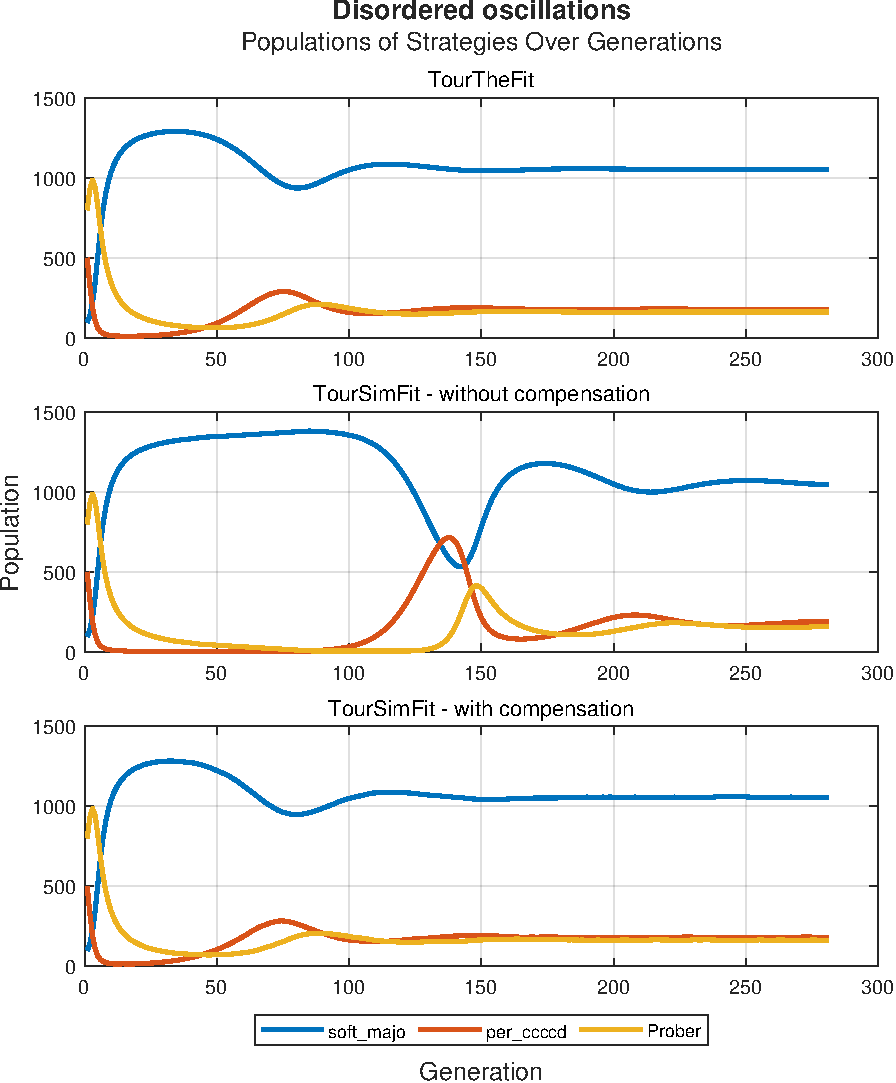
\includegraphics{Disordered oscillations.pdf}
	      \caption{Disordered oscillations}
	      \label{fig:2dmesh}
	\end{figure}
\section{Imitation Dynamics}

\subsection{Η συνάρτηση TourSimImi}

\subsubsection{1η Προσομοίωση}

\subsection{Η συνάρτηση TourTheImi}

\subsubsection{1η Προσομοίωση}

\section{Τελικά Συμπεράσματα}

\newpage
\listoffigures\addcontentsline{toc}{section}{Κατάλογος σχημάτων}
\end{document}